\begin{frame}
  \frametitle{What We Want}
  \framesubtitle{Versus What We Have}
  \begin{columns}


    \begin{column}{0.5\textwidth}
      What we think of as security
    
\includegraphics[width=1.0\textwidth]{safe}
  \end{column}


  \begin{column}{0.5\textwidth}
    \begin{center}
      What security actually is
    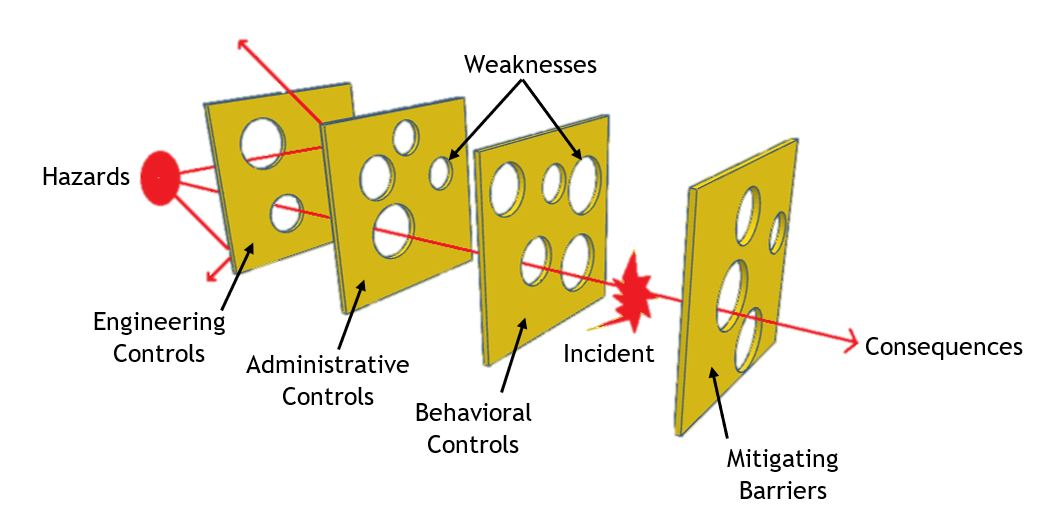
\includegraphics[width=1.4\textwidth]{SwissCheese}
    \end{center}

  \end{column}

  \end{columns}

  \note{\scriptsize{Security in a complex computer environment is an inter-layering of imperfect solutions. None of these security solutions is capable of stopping all, or even most attack vectors. And the larger the attack surface, the more such layers are necessary. Perfect security is an unattainable myth if we wish to retain a usable system capable of producing business value. Instead, our cybersecurity is dependent upon ensuring that each of the multiple layers of our defense-in-depth is as robust as is reasonably possible \parencite{janderDefenseindepthRoleAuthentication2018}, and that we focus on the weakest areas the most to achieve the greatest security posture. }}

\end{frame}
